\chapter{Background}

\section{Problem Derivation}
\subsection{Identified Problems}
\subsubsection{Slow Delta}
\begin{center}
    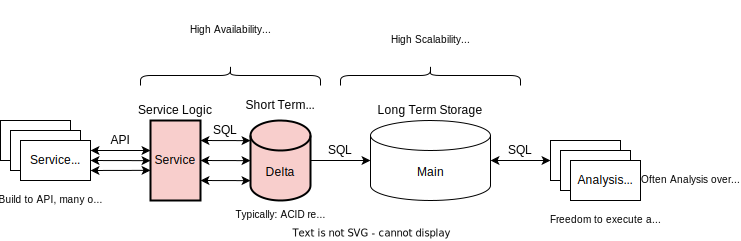
\includegraphics[scale=1.2]{_drawio/background/images/slow_delta.drawio.pdf}
\end{center}

\subsubsection{Complex State}
\begin{center}
    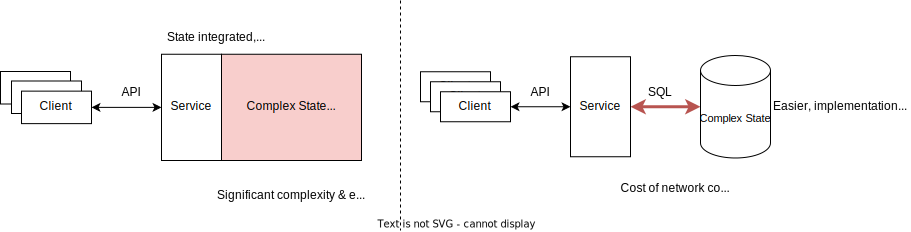
\includegraphics[scale=1.2]{_drawio/background/images/complex_service.drawio.pdf}
\end{center}
\subsubsection{Costly Analysis}
\begin{center}
    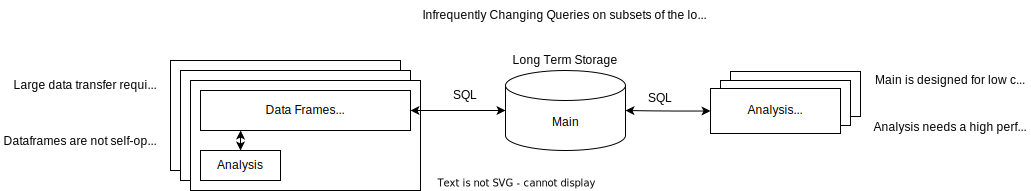
\includegraphics[scale=1.2]{_drawio/background/images/inefficient_analysis.drawio.pdf}
\end{center}

\subsection{Commonality}

\section{Embedded Databases}

\subsection{Dataframes}
\subsection{ArcticDB}
\subsection{DuckDB}
\subsection{SQLite}
\subsection{macroDB}

\section{Code Generation in Databases}
\subsection{VoltDB}
\subsection{SingleStore}

\section{Incremental View Maintenance}

\subsection{DBToaster}
DBToaster is an incremental view maintenance code generation tool, that generates C++, Spark (including a distributed spark target) and OCaml implementations from queries written in a subset of SQL.
\begin{center}
    \includegraphics[width=\textwidth]{_drawio/background/images/dbtoaster_system.drawio.pdf}
\end{center}

\begin{center}
    \begin{tabular}{l p{.8\textwidth}}
        \textbf{SQL} & blah \\
    \end{tabular}
\end{center}
\subsubsection{Incremental Calculus}
\subsubsection{Evaluation}




\subsection{Naiad/Materialize/Differential Dataflow}
\subsubsection{Evaluation}
\section{Domain Specific Languages}
\subsection{Language Integrated Queries}
\subsubsection{LINQ}

\subsubsection{sqlx}

\subsection{Rust Procedural Macros}

